\documentclass{llncs}
\usepackage[utf8]{inputenc}
\usepackage{booktabs}
\usepackage{rotating}
\RequirePackage{graphicx}
\RequirePackage[spanish]{babel}
\RequirePackage[utf8]{inputenc}
\selectlanguage{spanish}
\usepackage{verbatim} 


\newcommand{\mykeywords}[1]{\par\addvspace\baselineskip \noindent \textbf{Palabras Claves:} \enspace\ignorespaces#1}

\newtheorem{teo}{Teorema}

\begin{document}

\title{Sudoku Hidato}

\author{
  Masiel Villalba Carmenate \email{villalbamasiel@gmail.com}\institute{Facultad de Matem\'atica y Computaci\'on (MATCOM), \\Universidad de la Habana (UH), Cuba.}
  }

\titlerunning{Programaci\'on Declarativa} 
\authorrunning{Masiel Villalba Carmenate}


\maketitle

\section{Preliminares. Aleatoriedad}
La aleatoriedad se consigui\'o mediante el m\'odulo \texttt{System.Random}\cite{baeza} y las principales funciones empleadas fueron \texttt{random} para obtener un valor arbitrario, \texttt{randomR} para generar n\'umeros aleatorios en un rango y \texttt{randoms} para construir una secuencia infinita de valores aleatorios. Tal secuencia infinita es utilizada por casi todas las funciones de la implementaci\'on a partir de \'indices que indican cu\'al es el valor que les corresponde utilizar y ha sido primordial puesto que \texttt{random} y \texttt{randomR}~(Figura\ref{rand}) reciben ambos un objeto tipo \texttt{RandomGen}~(un generador \emph{random}) que puede construirse manualmente con la funci\'on \texttt{mkStdGen} a partir de un valor ``semilla'' donde, con motivo de la transparencia referencial de Haskell, debe de variar para que \texttt{mkStdGen} y por consiguiente, \texttt{random} y \texttt{randomR} devuelvan valores diferentes en cada llamado.

%que puede construirse manualmente con la funci\'on \texttt{mkStdGen} cuya signatura es \texttt{mkStdGen :: Int -> StdGen}
\section{Representaci\'on}
Los Hidatos han sido representados como una tripla $(M,I,F)$ donde $I$ es la posici\'on donde est\'a ubicado el valor m\'inimo del tablero, $F$ la posici\'on del valor m\'aximo y $M$ una matriz de $n$ filas y $m$ columnas donde:
\begin{itemize}
\item las casillas que deben de rellenarse para completar el sudoku tienen asignado valor -2,
\item las casillas con valor predefinido tienen un n\'umero arbitrario entre $1$ y $k$, donde se dice que $k$ es el \emph{tama\~no del hidato}\footnote{Se a mantenido el valor $1$ como el m\'inimo para generar todos los hidatos y el valor m\'aximo coincide con el tama\~no del mismo.},
\item existen casillas ``ficticias'' que sirven para simular la forma del Hidato y tienen  valor $-1$.
\end{itemize}

La Figura \ref{hidato} muestra un ejemplo de un Hidato con esta representaci\'on.

\begin{figure}
\begin{center}
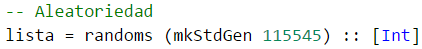
\includegraphics[width= .8\columnwidth]{figuras/lista}
\end{center}
\caption{Secuencia ``global'' de valores \emph{random} en la implementaci\'on. El valor que recibe \texttt{mkStdGen} para construirla puede ser cambiado manualmente por  cualquier otro.}
\label{listar}
\end{figure}

\begin{figure}
\begin{center}
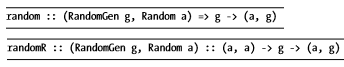
\includegraphics[width= .7\columnwidth]{figuras/rand}
\end{center}
\caption{Signatura de \texttt{random} y \texttt{randomR}. Tomado de \cite[p.191, p.194]{baeza}}
\label{rand}
\end{figure}

\begin{figure}
\begin{center}
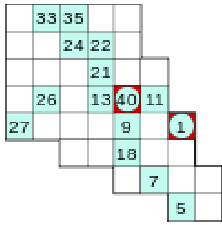
\includegraphics[width= 0.3\columnwidth]{figuras/sudoku}
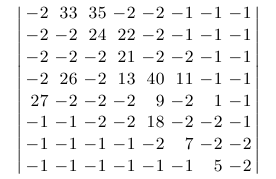
\includegraphics[width= 0.48\columnwidth]{figuras/matrep}
\end{center}
\caption{Sudoku Hidato de tama\~no 40 a la izquierda y su representaci\'on matricial a la derecha.}
\label{hidato}
\end{figure}





\begin{comment}
\begin{center}
$\left| 
\begin{array}{rrrrrrrr}
-2 & 33 & 35 & -2 & -2 & -1 & -1 & -1 \\
-2 & -2 & 24 & 22 & -2 & -1 & -1 & -1 \\
-2 & -2 & -2 & 21 & -2 & -2 & -1 & -1 \\
-2 & 26 & -2 & 13 & 40 & 11 & -1 & -1 \\
27 & -2 & -2 & -2 & 9 & -2 & 1 & -1 \\
-1 & -1 & -2 & -2 & 18 & -2 & -2 & -1 \\
-1 & -1 & -1 & -1 & -2 & 7 & -2 & -2 \\
-1 & -1 & -1 & -1 & -1 & -1 & 5 & -2
\end{array} 
\right|$
\end{center}
\end{comment}

\section{Generando Hidatos}
Esencialmente, el procedimiento que se realiza es generar una soluci\'on y a partir de ella elegir las casillas que se quedar\'an con valores prefijados. 

\subsection{Crear una soluci\'on}
Dado que un Hidato pudiera representarse tambi\'en como una secuencia de casillas que describen el ``camino'' que forma la secuencia de n\'umeros que comienza en 1 y termina en el tama\~no del Hidato, las soluciones se construyen mediante una idea recursiva: dada la posici\'on actual que se ocupa, cu\'al es el siguiente paso que se va a dar considerando las 8 opciones\footnote{Izquierda, derecha, arriba, abajo y los 4 movimientos en diagonal~(Figura \ref{movs}).} con las que se cuenta?
Esta elecci\'on se toma cada vez de manera aleatoria sobre el conjunto de las celdas vecinas:
\begin{itemize}
\item a las cuales no se les ha asignado ning\'un valor,
\item sobre aquellas que se salen de los l\'imites de la matriz actual. En este caso la nueva matriz que representa al Hidato tendr\'a una fila y/o columna m\'as respecto a la anterior, de forma tal que en ella la posici\'on seleccionada no sea un paso exterior~(Figura \ref{camino}). 
\end{itemize}


\begin{figure}
\begin{center}
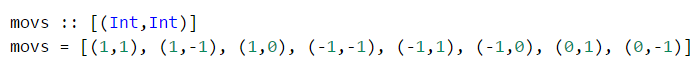
\includegraphics[width= 1\columnwidth]{figuras/movs}
\end{center}
\caption{Las 8 opciones de movimiento desde una casilla.}
\label{movs}
\end{figure}


\begin{figure}
\begin{center}
$\left| 
\begin{array}{r}
1
\end{array} 
\right|$
\end{center}

\begin{center}
$\left| 
\begin{array}{rr}
1 & 2
\end{array} 
\right|$
\end{center}

\begin{center}
$\left| 
\begin{array}{rrr}
1 & 2 & -1 \\
-1 & -1 & 3 \\
\end{array} 
\right|$
\end{center}
\caption{Aumento de la matriz seg\'un los pasos tomados. Al ubicar al $2$ en el tablero la nueva matriz contiene una columna m\'as a la derecha y al ubicar al $3$ aparece una nueva columna a la derecha y una fila m\'as.}
\label{camino}
\end{figure}

Se elige \'unicamente una casilla exterior si no existe ninguna vecina que est\'e vac\'ia para reforzar la ``densidad'' del sudoku. Se parte de la matriz que tiene una sola fila y una columna y se considera caso de parada cuando el valor que corresponde colocar es el del tama\~no que se ha previsto que tenga el Hidato.

\subsection{Elegir valores predeterminados}
Una vez construida una soluci\'on, se determina qu\'e celdas estar\'an vac\'ias y cu\'ales tendr\'an valores predeterminados. Al desarrollar la implementaci\'on, surgieron varias ideas:
\begin{itemize}
\item Elegir casillas aleatoriamente para prefijar: en este caso no se garantiza que el Hidato tenga soluci\'on \'unica.
\item Elegir qu\'e valores del tablero se prefijar\'an: concretamente cada vez que se elige arbitrariamente un n\'umero, se prefijan en el tablero su valor y el del sucesor de su sucesor, as\'i se restringe la cantidad de lugares que puede ocupar el n\'umero del centro. Aunque esta estrategia es menos r\'apida que la primera~(puesto que al determinar el valor a prefijar requiere detectar qu\'e posici\'on ocupa en la soluci\'on construida) y tampoco garantiza que la soluci\'on del Hidato sea \'unica, s\'i resuelve al menos que se reduzca la cantidad de soluciones.
\end{itemize}


Estas ideas se materializan con las funciones \texttt{select\_no\_empty} y\\ \texttt{select\_better\_no\_empty}~(Figura \ref{select}) respectivamente. Se rellenan el 35\% de las celdas, sin considerar las que contienen el valor m\'inimo y m\'aximo  del tablero que siempre ser\'an prefijadas. Puede ser que aumentar este porcentaje consiga garantizar la unicidad de la soluci\'on pero reducir\'ia la complejidad del ``juego''.

\begin{figure}
\begin{center}
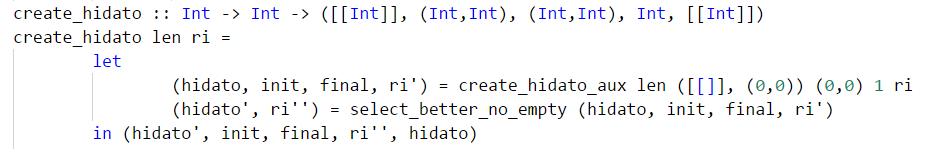
\includegraphics[width= 1\columnwidth]{figuras/createh}
\end{center}
\caption{Funci\'on mediante la cual se crea un Hidato. El par\'ametro \texttt{len} es el tama\~no del Hidato que se desea construir y \texttt{ri} es el \'indice de la lista de valores aleatorios a partir del cual se comienza a trabajar.}
\label{create}
\end{figure}




\begin{figure}
\begin{center}
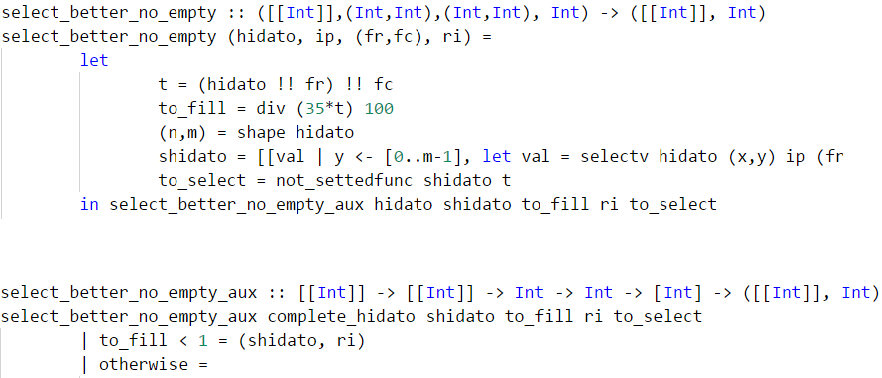
\includegraphics[width= 1\columnwidth]{figuras/select}
\end{center}
\caption{Segmentos de las funciones mediante las que se determinan los valores prefijados.}
\label{select}
\end{figure}
\section{Solucionando Hidatos}
Para conocer la cantidad de soluciones de un Hidato dado, la funci\'on que las detecta explota todas las posibilidades de manera exhaustiva~(Figura \ref{solver}). La idea en esencia es recursiva y define que, dada una posici\'on del tablero, las soluciones del mismo ser\'an las que se obtengan de ubicar el siguiente valor del camino en cada una de las casillas que se pueda colocar desde la posici\'on actual. Se parte de la posici\'on donde est\'a ubicado el valor m\'inimo del tablero y los casos base son aquellos en los que el pr\'oximo valor del camino es el m\'aximo n\'umero y se est\'a en una posici\'on vecina a su ubicaci\'on.


Claro que se puede modificar el procedimiento para que la recursi\'on termine cuando se encuentre una soluci\'on, pero se procedi\'o de esta manera para evaluar la estrategia de prefijar los valores del Hidato. De cualquier manera, el problema de resolver un Hidato se puede reducir al Problema de Satisfacci\'on Booleana~(SAT, conocido as\'i en ingl\'es por su abreviatura) el cual es considerado un problema NP-completo\cite{serio}.

\section{Inicio del ``juego''}
Mediante la funci\'on \texttt{hidatos\_list} con signatura \texttt{hidatos\_list :: Int -> Int -> Int -> String}~(\texttt{hidatos\_list n len ri}) se especifica que se desea generar y solucionar $n$ Hidatos de tama\~no $len$. Mediante funciones definidas en \texttt{Utils.hs} se imprimen el Hidato y todas sus soluciones. Al valor $ri$ en este llamado debe asign\'arsele valor $0$ como se observa en la Figura \ref{main} para comenzar a utilizar la secuencia de n\'umeros aleatorios desde el comienzo.

\begin{figure}
\begin{center}
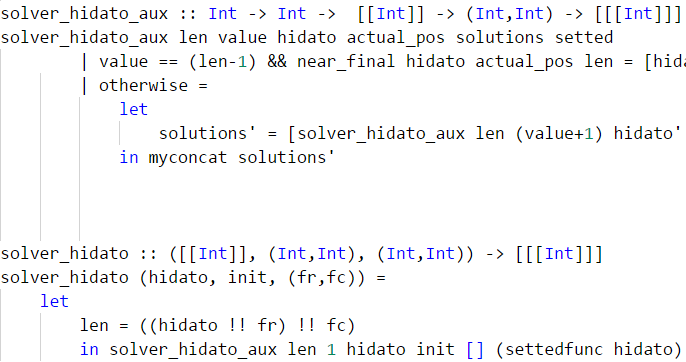
\includegraphics[width= 1\columnwidth]{figuras/solver}
\end{center}
\caption{Segmentos de las funciones mediante las que se les da soluci\'on al Hidato.}
\label{solver}
\end{figure}

\begin{figure}
\begin{center}
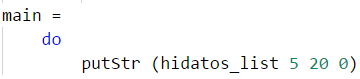
\includegraphics[width= .5\columnwidth]{figuras/main}
\end{center}
\caption{Ejemplo de invocaci\'on al ``juego'' en \texttt{Main.hs}.}
\label{main}
\end{figure}


\begin{figure}
\begin{center}
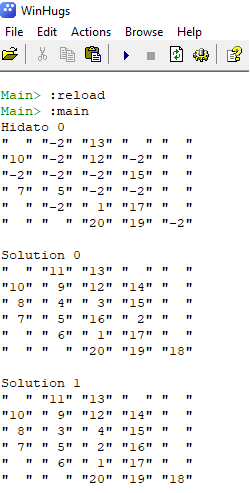
\includegraphics[width= .5\columnwidth]{figuras/corrida}
\end{center}
\caption{Secci\'on de la salida del ``juego'' con la invocaci\'on de la Figura \ref{main}.}
\label{corrida}
\end{figure}
\begin{thebibliography}{5}  
\bibitem{baeza}
    Lipovaca, Miran: 
    Learn you a Haskell for a great good!,
    Cap9, Randomness,
    2011.
    
\bibitem{serio}
	Barto{\v{s}}, Samuel:
	Effective encoding of the Hidato and Numbrix puzzles to their CNF representation,
	Univerzita Karlova, Matematicko-fyzik{\'a}ln{\'\i} fakulta,
	2014
\end{thebibliography}
\end{document}